% Template for IGARSS-2020 paper; to be used with:
%          spconf.sty  - LaTeX style file, and
%          IEEEbib.bst - IEEE bibliography style file.
% --------------------------------------------------------------------------
\documentclass{article}
\usepackage{spconf,amsmath,epsfig}
\usepackage{subcaption}
\usepackage{multirow}
% Example definitions.
% --------------------
\def\x{{\mathbf x}}
\def\L{{\cal L}}

% Title.
% ------
\title{USING THE GAF TRANSFORM AND MODIS TIME-SERIES TO PERFORM LANDCOVER CLASSIFICATION AND CHANGE DETECTION}
%
% Single address.
% ---------------
\name{Author(s) Name(s)\thanks{Thanks to XYZ agency for funding.}}
\address{Author Affiliation(s)}
%
% For example:
% ------------
%\address{School\\
%	Department\\
%	Address}
%
% Two addresses (uncomment and modify for two-address case).
% ----------------------------------------------------------
%\twoauthors
%  {A. Author-one, B. Author-two\sthanks{Thanks to XYZ agency for funding.}}
%	{School A-B\\
%	Department A-B\\
%	Address A-B}
%  {C. Author-three, D. Author-four\sthanks{The fourth author performed the work
%	while at ...}}
%	{School C-D\\
%	Department C-D\\
%	Address C-D}
%
\begin{document}
%\ninept
%
\maketitle
%
\begin{abstract}
The abstract should appear at the top of the left-hand column of text, about
0.5 inch (12 mm) below the title area and no more than 3.125 inches (80 mm) in
length.  Leave a 0.5 inch (12 mm) space between the end of the abstract and the
beginning of the main text.  The abstract should contain about 100 to 150
words, and should be identical to the abstract text submitted electronically
along with the paper cover sheet.  All manuscripts must be in English, printed
in black ink.
\end{abstract}
%
\begin{keywords}
One, two, three, four, five
\end{keywords}
%
\section{Introduction}
\label{sec:intro}
The field of computer vision has changed dramatically over the last few years due to the success of Convolutional Neural Networks (CNNs) and deep learning. Recently, it was proposed to encode time-series as images so that the capability of CNNs to perform image classification could also be applied to the problem of time-series classification. One possible time-series encoding scheme is the Gramian Angular Field (GAF) transform. GAF images are formed using polar coordinates and ultimately take the form of a Gramian matrix, whose entries are the trigonometric sum of observations recorded at different time indices. This encoding scheme has succesfully been applied within the remote sensing field. Dias et al used the GAF transform (and other transforms), Moderate Resolution Imaging Spectroradiometer (MODIS) time-series and existing CNN models to succesfully detect eucalyptus plantations. Their CNN based solution outperformed the conventional approaches they compared against. In this paper we will investigate whether MODIS time-series and the GAF transfrom can be utilized for detecting settlement expansion. Settlement expansion is one of the most pervasive forms of landcover change in sub saharan Africa. It is, therefore, of the utmost importance to find strategies and algorithms that will allow us to effectively monitor the growth of settlements in Africa. In this paper, however, we will restrict ourselves to a case study in the Gauteng province of South Africa. It is also woth pointing out that in this paper we alse  

%Given this background, let us list the  contributions that we make in this paper: 
%\begin{itemize}
% \item Our indepenent study corroborates the study made by Dias et al, i.e. we have confirmed that the GAF transform is a usefull encoding scheme that can be used for pixel-based land cover classification. 
% \item We show that the GAF transform can be utilized for detecting settlement expasion.
% \item We show that the GAF transform can not only be used for pixel based land cover classification, but also for detecting land cover change.
% \item We show that is the classification problem at hand is seperable enough
%\end{itemize}



In addition to investigating wheter the GAF transform can be utilized for detecting settlement expansion, the current paper also makes the following unique contributions:

we also Let us now expand on the unique contributions of the current paper in a bit Expanding on the , the unique contributions of the current paper are:
\begin{itemize}
 \item 
\end{itemize}




GAF images are rep-resented as a Gramian matrix where each element is thetrigonometric sum (i.e., superposition of directions) be-tween different time intervals


such an approach is to use the GAF transform to encode time-series as images for classification The  transform  



As an example of it, CNNs can easily distinguish photographs of dogs and cats  


These guidelines include complete descriptions of the fonts, spacing, and
related information for producing your proceedings manuscripts. Please follow
them and if you have any questions, direct them to Conference Management
Services, Inc.: Phone +1-979-846-6800 or Fax +1-979-846-6900 or email
to \verb+papers@igarss2020.org+.

\section{Formatting your paper}
\label{sec:format}

All printed material, including text, illustrations, and charts, must be kept
within a print area of 7 inches (178 mm) wide by 9 inches (229 mm) high. Do
not write or print anything outside the print area. The top margin must be 1
inch (25 mm), except for the title page, and the left margin must be 0.75 inch
(19 mm).  All {\it text} must be in a two-column format. Columns are to be 3.39
inches (86 mm) wide, with a 0.24 inch (6 mm) space between them. Text must be
fully justified.

\section{PAGE TITLE SECTION}
\label{sec:pagestyle}

The paper title (on the first page) should begin 1.38 inches (35 mm) from the
top edge of the page, centered, completely capitalized, and in Times 14-point,
boldface type.  The authors' name(s) and affiliation(s) appear below the title
in capital and lower case letters.  Papers with multiple authors and
affiliations may require two or more lines for this information.

\section{TYPE-STYLE AND FONTS}
\label{sec:typestyle}

To achieve the best rendering in the proceedings, we
strongly encourage you to use Times-Roman font.  In addition, this will give
the proceedings a more uniform look.  Use a font that is no smaller than ten
point type throughout the paper, including figure captions.

In ten point type font, capital letters are 2 mm high.  If you use the
smallest point size, there should be no more than 3.2 lines/cm (8 lines/inch)
vertically.  This is a minimum spacing; 2.75 lines/cm (7 lines/inch) will make
the paper much more readable.  Larger type sizes require correspondingly larger
vertical spacing.  Please do not double-space your paper.  True-Type 1 fonts
are preferred.

The first paragraph in each section should not be indented, but all the
following paragraphs within the section should be indented as these paragraphs
demonstrate.

\section{MAJOR HEADINGS}
\label{sec:majhead}

Major headings, for example, "1. Introduction", should appear in all capital
letters, bold face if possible, centered in the column, with one blank line
before, and one blank line after. Use a period (".") after the heading number,
not a colon.

\subsection{Subheadings}
\label{ssec:subhead}

Subheadings should appear in lower case (initial word capitalized) in
boldface.  They should start at the left margin on a separate line.
 
\subsubsection{Sub-subheadings}
\label{sssec:subsubhead}

Sub-subheadings, as in this paragraph, are discouraged. However, if you
must use them, they should appear in lower case (initial word
capitalized) and start at the left margin on a separate line, with paragraph
text beginning on the following line.  They should be in italics.

\section{PRINTING YOUR PAPER}
\label{sec:print}

Print your properly formatted text on high-quality, 8.5 x 11-inch white printer
paper. A4 paper is also acceptable, but please leave the extra 0.5 inch (12 mm)
empty at the BOTTOM of the page and follow the top and left margins as
specified.  If the last page of your paper is only partially filled, arrange
the columns so that they are evenly balanced if possible, rather than having
one long column.

In LaTeX, to start a new column (but not a new page) and help balance the
last-page column lengths, you can use the command ``$\backslash$pagebreak'' as
demonstrated on this page (see the LaTeX source below).

\section{PAGE NUMBERING}
\label{sec:page}

Please do {\bf not} paginate your paper.  Page numbers, session numbers, and
conference identification will be inserted when the paper is included in the
proceedings.

\section{ILLUSTRATIONS, GRAPHS, AND PHOTOGRAPHS}
\label{sec:illust}

Illustrations must appear within the designated margins.  They may span the two
columns.  If possible, position illustrations at the top of columns, rather
than in the middle or at the bottom.  Caption and number every illustration.
All illustrations should be clear wwhen printed on a black-only printer. Color
may be used.

Since there are many ways, often incompatible, of including images (e.g., with
experimental results) in a LaTeX document, below is an example of how to do
this \cite{Lamp86}.

% Below is an example of how to insert images. Delete the ``\vspace'' line,
% uncomment the preceding line ``\centerline...'' and replace ``imageX.ps''
% with a suitable PostScript file name.
% -------------------------------------------------------------------------
\begin{table}
\begin{tabular}{ |l|c c c| }
\hline
%\multicolumn{3}{ |c| }{Team sheet} \\
& & v & s\\
\hline
\multirow{2}{*}{PCA} & \emph{v} & 93.63$\pm$1.58&6.37\\
& \emph{s}& 0.6& 99.41\%$\pm$0.39\\
\hline
\multirow{2}{*}{GAF} & \emph{v} & 99.42$\pm$0.58&0.58\\
& \emph{s}& 0.77& 99.23\%$\pm$0.64\\
\hline
\hline
& & nc & c\\
\hline
\multirow{2}{*}{Differencing} & \emph{nc} & 85.47 & 14.53\\
& \emph{c}& 16.11 & 83.89\\
\multirow{2}{*}{GAF} & \emph{nc} & 99.2$\pm$0.71 & 0.8\\
& \emph{c}& 0.01 & 99.9$\pm$0.17\\
%Goalkeeper & GK & Paul Robinson \\ \hline
%\multirow{4}{*}{Defenders} & LB & Lucas Radebe \\
% & DC & Michael Duburry \\
% & DC & Dominic Matteo \\
% & RB & Didier Domi \\ \hline
%\multirow{3}{*}{Midfielders} & MC & David Batty \\
% & MC & Eirik Bakke \\
% & MC & Jody Morris \\ \hline
%Forward & FW & Jamie McMaster \\ \hline
%\multirow{2}{*}{Strikers} & ST & Alan Smith \\
% & ST & Mark Viduka \\
\hline
\end{tabular}
\caption{xxx}
\label{tab:cm}
\end{table}


\begin{figure}[htb]

\begin{minipage}[b]{1.0\linewidth}
  \centering
% \centerline{\epsfig{figure=image1.ps,width=8.5cm}}
  \vspace{2.0cm}
  \centerline{(a) Result 1}\medskip
\end{minipage}
%
\begin{minipage}[b]{.48\linewidth}
  \centering
% \centerline{\epsfig{figure=image3.ps,width=4.0cm}}
  \vspace{1.5cm}
  \centerline{(b) Results 3}\medskip
\end{minipage}
\hfill
\begin{minipage}[b]{0.48\linewidth}
  \centering
% \centerline{\epsfig{figure=image4.ps,width=4.0cm}}
  \vspace{1.5cm}
  \centerline{(c) Result 4}\medskip
\end{minipage}
%
\caption{Example of placing a figure with experimental results.}
\label{fig:res}
%
\end{figure}

\begin{figure}
 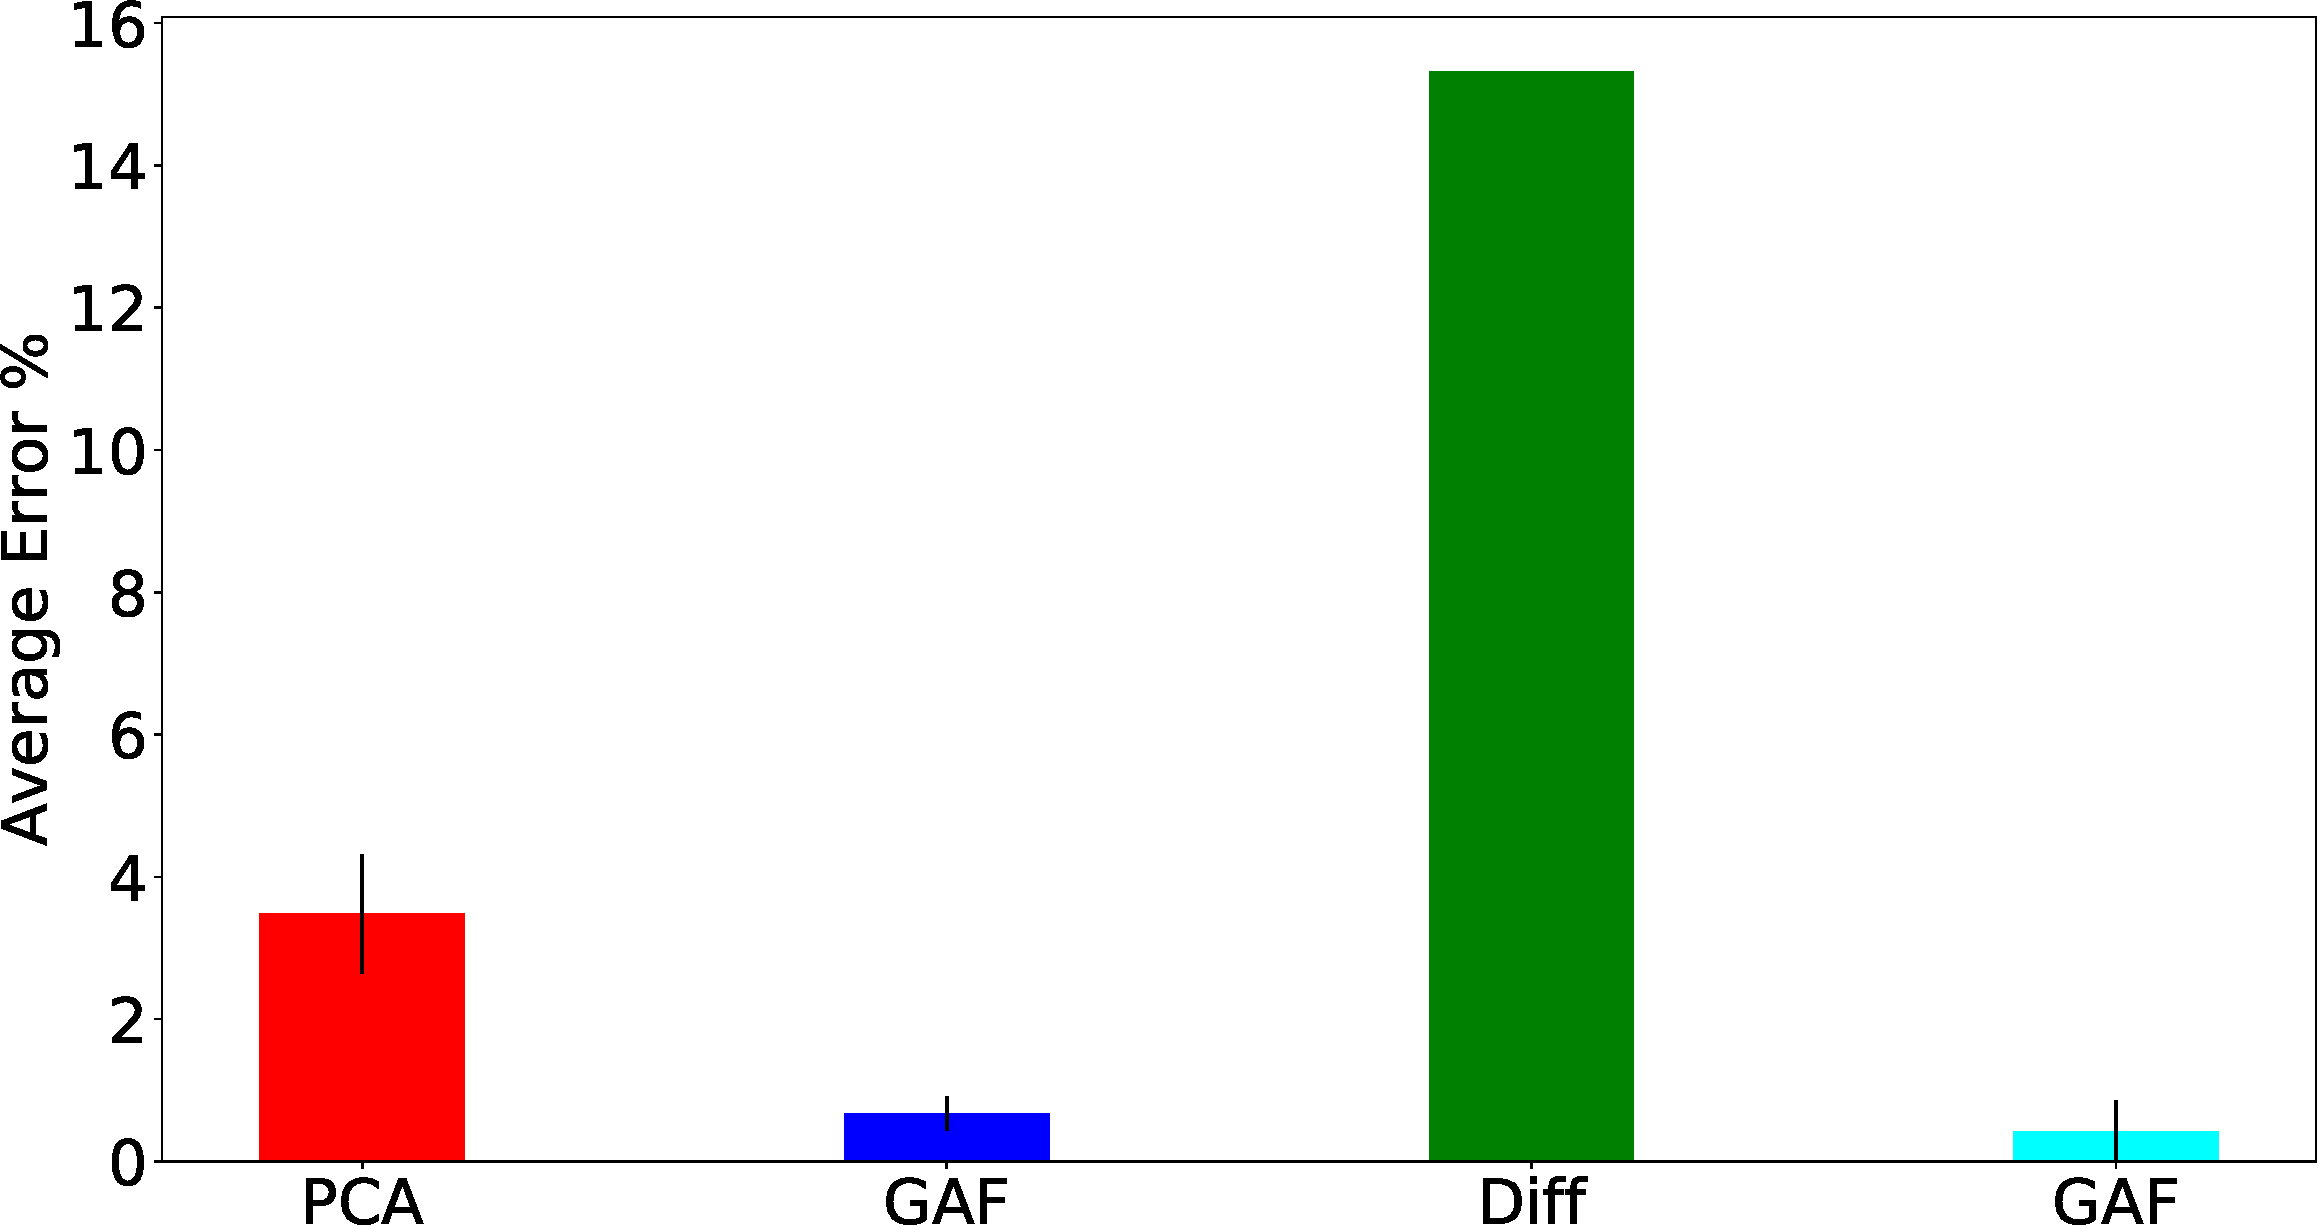
\includegraphics[width=0.48\textwidth]{results-crop.pdf}
 \label{fig:results}
 \caption{Test}
\end{figure}


\begin{figure*}[h] 
  \begin{subfigure}[b]{0.5\linewidth}
    \centering
    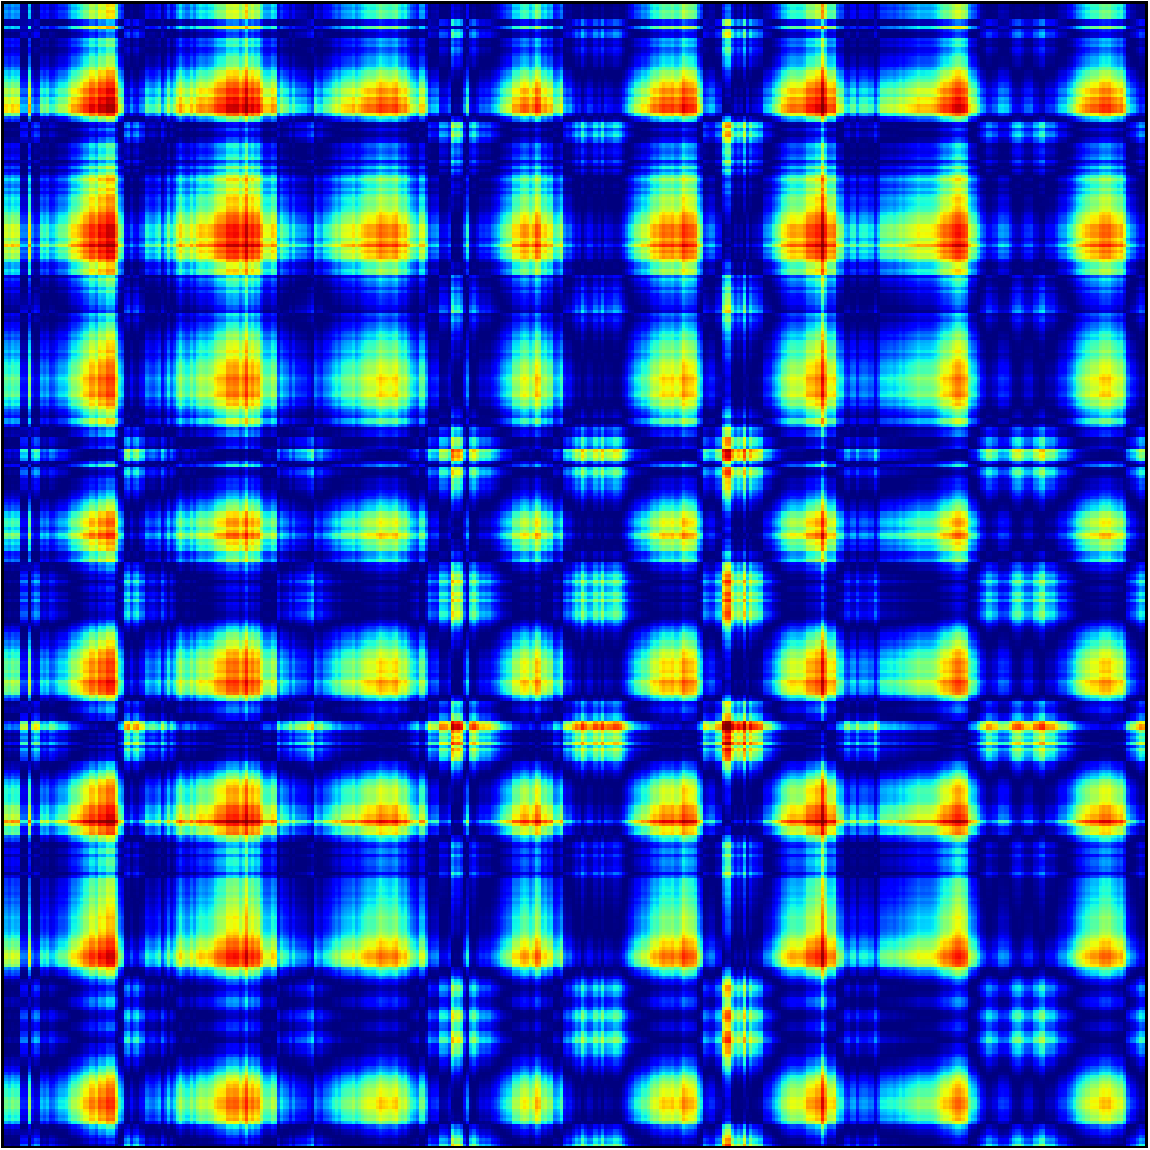
\includegraphics[width=0.89\linewidth]{veg-crop.pdf} 
    \caption{Vegetation} 
    \label{fig7:a} 
    \vspace{6ex}
  \end{subfigure}%% 
  \begin{subfigure}[b]{0.5\linewidth}
    \centering
    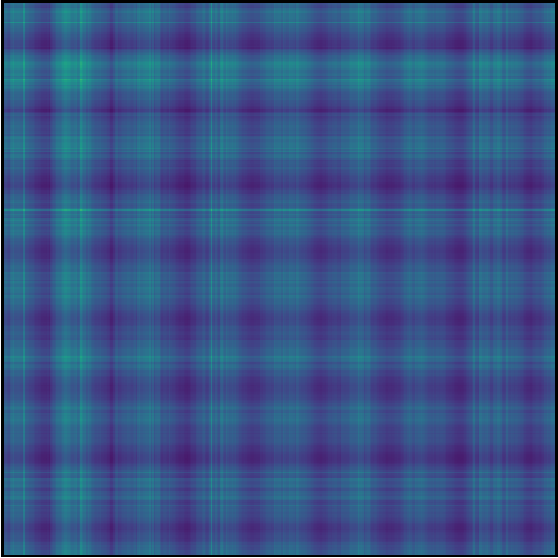
\includegraphics[width=0.89\textwidth]{bwt-crop.pdf} 
    \caption{Settlement} 
    \label{fig7:b} 
    \vspace{6ex}
    \end{subfigure} 
    %\vspace{13ex}
  \begin{subfigure}[b]{0.5\linewidth}
    \centering
    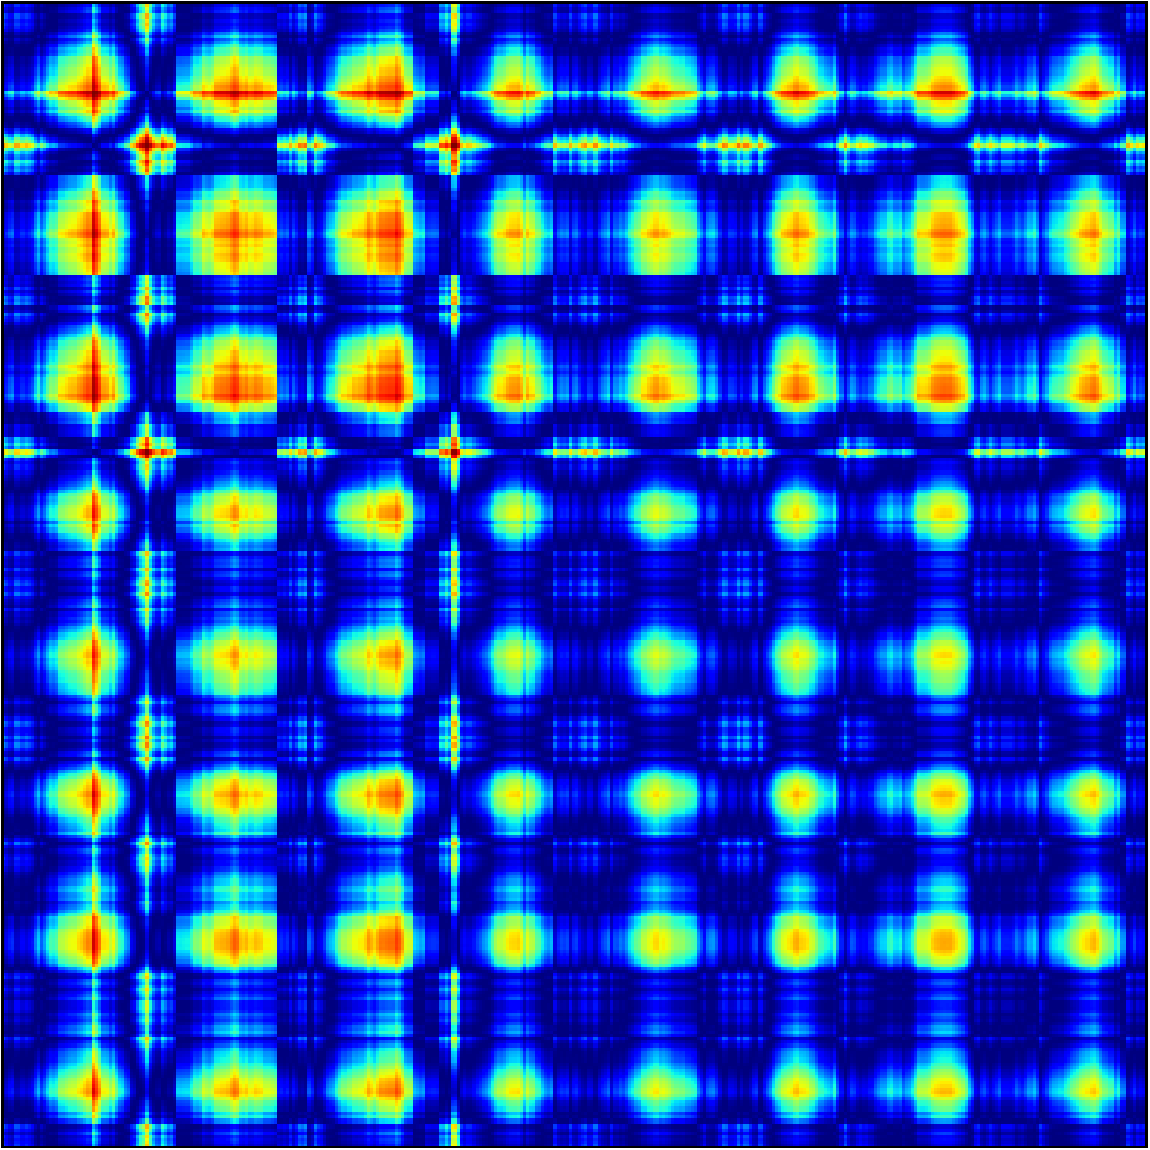
\includegraphics[width=0.89\textwidth]{sim_c-crop.pdf} 
    \caption{Simulated Change} 
    \label{fig7:c} 
  \end{subfigure}%%
  \begin{subfigure}[b]{0.5\linewidth}
    \centering
    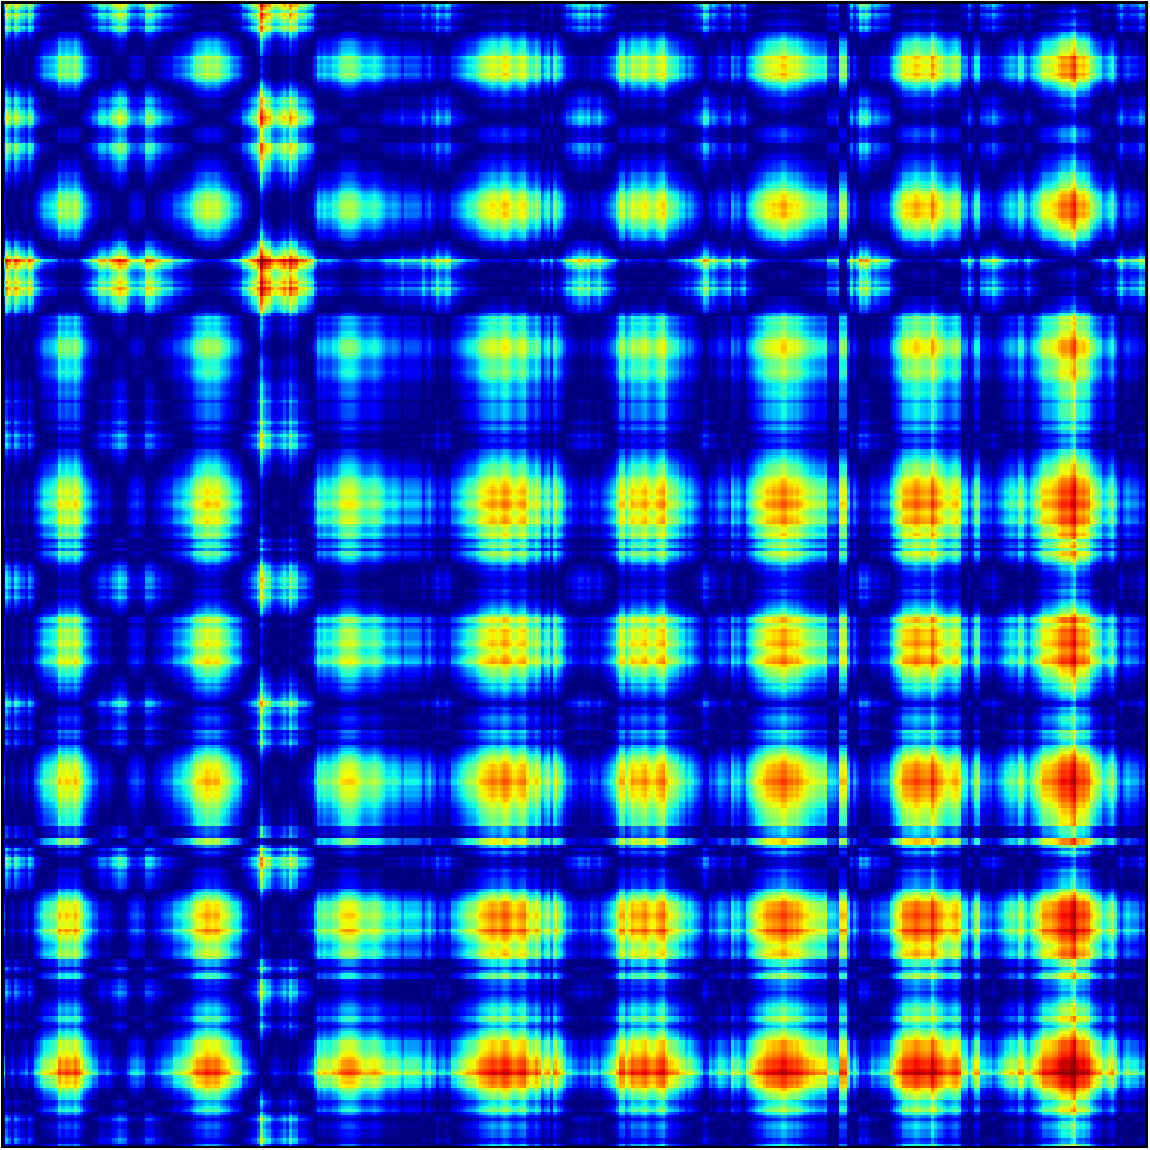
\includegraphics[width=0.89\textwidth]{real_c-crop.pdf} 
    \caption{Real Change} 
    \label{fig7:d} 
  \end{subfigure} 
  \label{fig7} 
  \caption{The classification accuracy (\%) results obtained if we employ the supervised (top left) and the unsupervised (top right) sequential classification approaches presented in Section~\ref{sec:sprt} to classify (cluster) the dataset presented in Section~\ref{sec:data}. The classification accuracy results obtained by applying $k$-means (bottom left) and GMM (bottom-right) to the the dataset presented in Section~\ref{sec:data} are also presented. The supervised approach outperforms the unsupervised approach as is expected. Note, the unsupervised sequential approach, however, outperforms traditional $k$-means.}
  \label{fig:results}
\end{figure*}






% To start a new column (but not a new page) and help balance the last-page
% column length use \vfill\pagebreak.
% -------------------------------------------------------------------------
\vfill
\pagebreak




\section{FOOTNOTES}
\label{sec:foot}

Use footnotes sparingly (or not at all!) and place them at the bottom of the
column on the page on which they are referenced. Use Times 9-point type,
single-spaced. To help your readers, avoid using footnotes altogether and
include necessary peripheral observations in the text (within parentheses, if
you prefer, as in this sentence).


\section{COPYRIGHT FORMS}
\label{sec:copyright}

You must also electronically sign the IEEE copyright transfer
form when you submit your paper. We {\bf must} have this form
before your paper can be sent to the reviewers or published in
the proceedings. The copyright form is provided through the IEEE
website for electronic signature. A link is provided upon
submission of the manuscript to enter the IEEE Electronic
Copyright Form system.

\section{REFERENCES}
\label{sec:ref}

List and number all bibliographical references at the end of the paper.  The references can be numbered in alphabetic order or in order of appearance in the document.  When referring to them in the text, type the corresponding reference number in square brackets as shown at the end of this sentence \cite{C2}.

% References should be produced using the bibtex program from suitable
% BiBTeX files (here: strings, refs, manuals). The IEEEbib.bst bibliography
% style file from IEEE produces unsorted bibliography list.
% -------------------------------------------------------------------------
\bibliographystyle{IEEEbib}
\bibliography{strings,refs}

\end{document}
